\documentclass[
  captions=tableheading,
  bibliography=totoc, 
  titepage=firstiscover,
]{scrartcl}

\usepackage{blindtext} %neuer input

\usepackage{longtable} % Tabellen über mehrere Seiten

\usepackage[utf8]{inputenc} %neuer input

\usepackage{scrhack}

\usepackage[aux]{rerunfilecheck} %Warnung falls nochmal kompiliert werden muss

\usepackage{fontspec} %Fonteinstellungen

\recalctypearea{}

\usepackage[main=ngerman]{babel} %deutsche Spracheinstellung

\usepackage{ragged2e} %neuer input

\usepackage{amsmath, nccmath}

\usepackage{amssymb} %viele mathe Symbole

\usepackage{mathtools} %Erweiterungen für amsmath


\DeclarePairedDelimiter{\abs}{\lvert}{\rvert}
\DeclarePairedDelimiter{\norm}{\lVert}{\rVert}

\DeclarePairedDelimiter{\bra}{\langle}{\rvert}
\DeclarePairedDelimiter{\ket}{\lvert}{\rangle}

\DeclarePairedDelimiterX{\braket}[2]{\langle}{\rangle}{
#1 \delimsize| #2
}

\NewDocumentCommand \dif {m}
{
\mathinner{\symup{d} #1}
}


\usepackage[
  math-style=ISO,
  bold-style=ISO,
  sans-style=italic,
  nabla=upright,
  partial=upright,
  warnings-off={
    mathtools-colon,
    mathtools-overbracket,
  },
]{unicode-math}

\setmathfont{Latin Modern Math}
\setmathfont{XITS Math}[range={scr, bfscr}]
\setmathfont{XITS Math}[range={cal, bfcal}, StylisticSet=1]


\usepackage[
  locale=DE,
  separate-uncertainty=true,
  per-mode=reciprocal,
  output-decimal-marker={,},
]{siunitx}

\usepackage[autostyle]{csquotes} %richtige Anführungszeichen

\usepackage{xfrac}

\usepackage{float}

\floatplacement{figure}{htbp}

\floatplacement{table}{htbp}

\usepackage[ %floats innerhalb einer section halten
  section,   %floats innerhalb er section halten
  below,     %unterhalb der Section aber auf der selben Seite ist ok
]{placeins}

\usepackage[
  labelfont=bf,
  font=small,
  width=0.9\textwidth,
]{caption}

\usepackage{subcaption} %subfigure, subtable, subref

\usepackage{graphicx}

\usepackage{grffile}

\usepackage{booktabs}

\usepackage{microtype} %Verbesserungen am Schriftbild

\usepackage[
backend=biber,
]{biblatex}

\addbibresource{../lit.bib}

\usepackage[ %Hyperlinks im Dokument
  german,
  unicode,
  pdfusetitle,
  pdfcreator={},
  pdfproducer={},
]{hyperref}

\usepackage{bookmark}

\usepackage[shortcuts]{extdash}

%\usepackage{warpcol}


\begin{document}
    \title{ATP Übungsblatt 9}
    \author{  
    Tobias Rücker\\
    \texorpdfstring{\href{mailto:tobias.ruecker@tu-dortmund.de}{tobias.ruecker@tu-dortmund.de}
    \and}{,} 
    Paul Störbrock\\
    \texorpdfstring{\href{mailto:paul.stoerbrock@tu-dortmund.de}{paul.stoerbrock@tu-dortmund.de}}{}
    }
\maketitle
\center{\Large Abgabegruppe: \textbf{Mittw. 10-12 Uhr}}
\thispagestyle{empty}

\newpage
\tableofcontents
\thispagestyle{empty}
\newpage

\setcounter{page}{1}

\section{Aufgabe 25}
\begin{figure}[H]
    \centering
    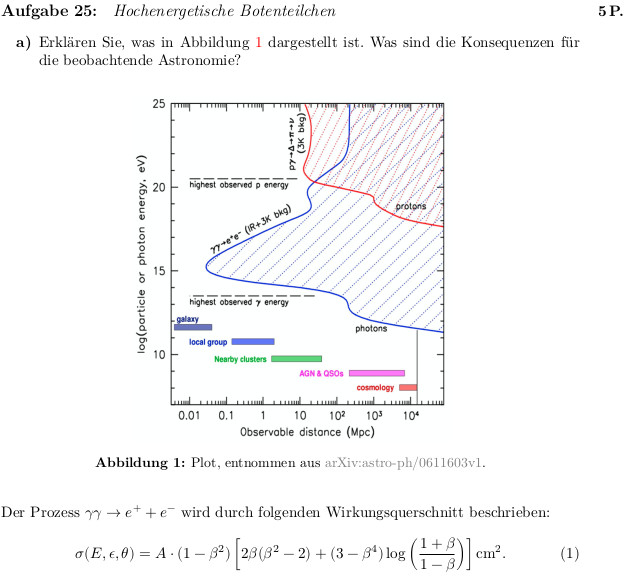
\includegraphics[width=\textwidth]{images/ex25_1.jpg}
\end{figure}
\begin{figure}[H]
    \centering
    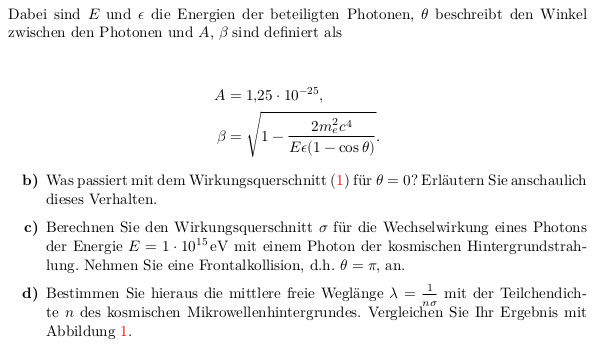
\includegraphics[width=\textwidth]{images/ex25_2.jpg}
\end{figure}


\subsection{a)}

    \flushleft{In\;}\justifying der Abbildung 1 wird die Energie der kosmischen Strahlung gegen die Entfernung zur Erde dargestellt. Die Distanz zur Erde beschreibt die
    Entfernung, aus welcher Protonen oder Photonen noch gemessen werden können. Außerdem sind verschiedene Distanzen farbig hinterlegt. Die höchste beobachtete 
    Photonen oder Protonen Energie ist eingezeichnet, sowie die Prozesse, die die Reichweite der Teilchen einschränken (Paarbildung und GZK-Cutoff).\\
    Photonen:\\
    Die höchste gemessene Energie eines Photons liegt bei ca. $10^{^13.5}$\SI{}{\electronvolt}. Bei höheren Energien kommt es zur Paarbildung, die besonders stark bei ca. 
    $10^{15}$\SI{}{\electronvolt} ist. Der $10^{15}$\SI{}{\electronvolt} Bereich kann laut Graphik nur innerhalb der Milchstraße gemssen werden. Oberhalb diesen Bereichs
    wird die Reichweite wieder größer. Deshalb können ab $10^{16}$\SI{}{\electronvolt} Protonen wieder in lokalen Gruppen, ab $10^{17.5}$\SI{}{\electronvolt} in nahen
    Galaxienclustern und ab $10^{22}$\SI{}{\electronvolt} in AGNs beobachtet werden. Bei $10^{22}$\SI{}{\electronvolt} ist die maximale Reichweite der hochenergetischen 
    Photonen. Im niederenergetischen Bereich $10^{11.5}$\SI{}{\electronvolt}, also vor der Paarbildung, können Photonen jedoch noch bei kosmologischen Distanzen beobachtet 
    werden.\\
    Protonen:\\
    Die höchste gemessene Energie eines Photons liegt bei ca. $10^{20.5}$\SI{}{\electronvolt}. Der GZK-Cutoff findet hier ab einer Energie von $10^{21}$\SI{}{\electronvolt}
    statt und reduziert die Reichweite auf die Distanz von lokalen Galaxienclustern.\\
    Die beobachtende Astronomie wird durch die Paarbildung und dem GZK-Cutoff bei hohen Energien auf relativ geringe Distanzen eingeschränkt. 


\subsection{b)}

    \flushleft{Für\;}\justifying $\theta=0$ divergiert der Bruch unter der Wurzel des $\beta$:
    \begin{align}
        \beta &=  \sqrt{ \underbrace{1- \frac{2m_e^2 c^4}{E\epsilon (1-\cos(\theta))}}_{<0}} \qquad \frac{2m_e^2 c^4}{0} \to \infty
        \intertext{
            \flushleft{Demnach\;}\justifying wird $\beta$ komplex.
        }
        1- \frac{2m_e^2 c^4}{E\epsilon (1-\cos(\theta))} &<0 \Leftrightarrow 1< \frac{2m_e^2 c^4}{E\epsilon (1-\cos(\theta))}\\
        1-\cos(\theta) &< \frac{2m_e^2 c^4}{E\epsilon}\\
        \cos(\theta) &> 1-\frac{2m_e^2 c^4}{E\epsilon} \qquad \left(\text{für}\; 0\leq \theta \leq \pi \to \cos(\theta) >x \Leftrightarrow \theta < \arccos(x) \right)\\
        \theta &< \arccos\left( 1-\frac{2m_e^2 c^4}{E\epsilon} \right) 
    \end{align}

\subsection{c)}

    \begin{align}
        \sigma(E,\epsilon, \theta) &= A(1-\beta^2) \left[ 2\beta(\beta^2 -2) + (3-\beta^4) \log\left( \frac{1+\beta}{1-\beta} \right) \right]\\
        \beta &= \sqrt{1- \frac{2m_e^2 c^4}{E\epsilon (1-\cos(\theta))}} \approx 0.8798\\
        \sigma(E,\epsilon, \theta) &= 2.0051 \cdot 10^{-30} \text{\SI{}{\meter\squared}}
    \end{align}


\subsection{d)}

    \begin{align}
        \lambda &= \frac{1}{n\sigma}
        \intertext{
            \flushleft{$n$\;}\justifying klauen wir uns aus Übung 8: $n=3.98 \cdot 10^8 \frac{1}{\text{\SI{}{\meter\squared}}}$
        }
        \Rightarrow \lambda &= 1.253 \cdot 10^{21} \text{\SI{}{\meter}} = 40.606 \text{kpc}
    \end{align}



\section{Aufgabe 26}
\begin{figure}[H]
    \centering
    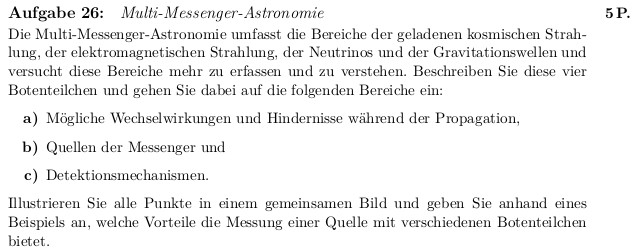
\includegraphics[width=\textwidth]{images/ex26.jpg}
\end{figure}

\begin{figure}[H]
    \centering
    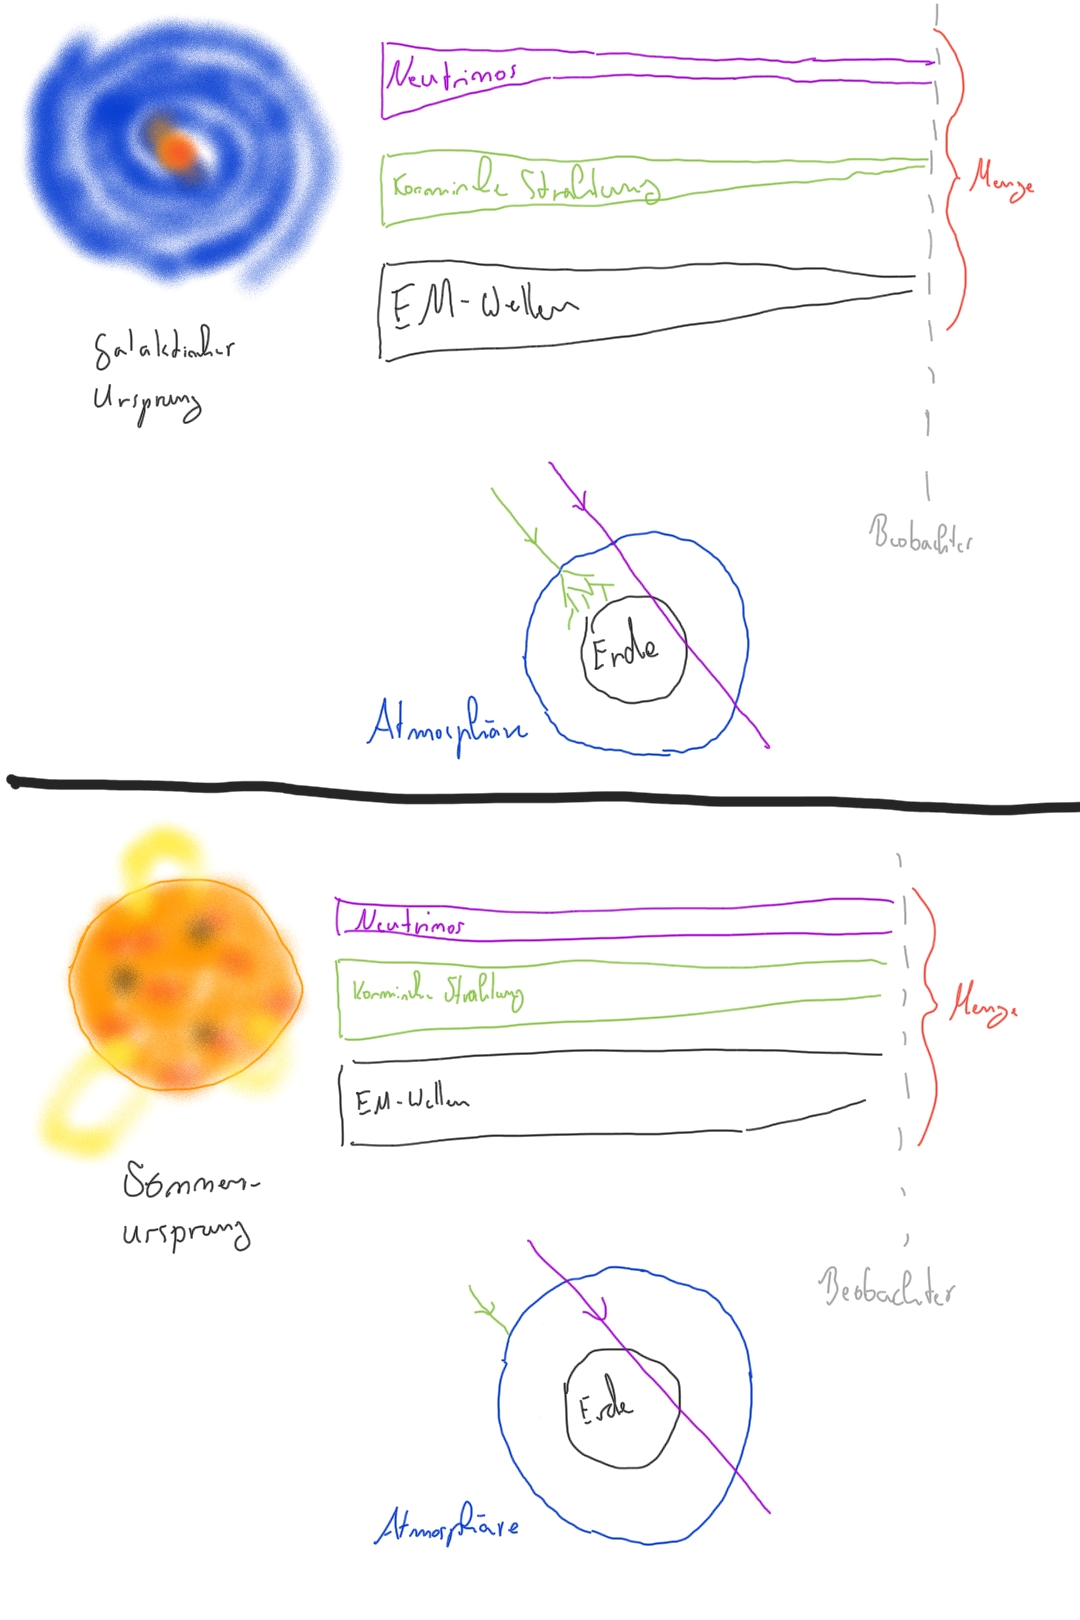
\includegraphics[width=0.75\textwidth]{images/Messenger.jpg}
\end{figure}


Kosmische Strahlung:\\
Unter kosmischer Strahlung versteht man eine Teilchenstrahlung, welche von Sternen und Galaxien 
ermittiert werde. Dabei handelt es sich großteils um Protonen, aber auch Elektronen und ionisierte
Kerne. Diese treffen auf die Erdatmosphäre und erzeugen dort einen Teilchenschauer,
wobei der bei Protonen ausgedenter ist, während Elektronen einen Linienförmigen Schauer
erzeugen. Auf dem Weg von den Quellen treffen diese Teilchen auf Masseansammlungen
wie Gaswolken und wechselwirken mit den dortigen Teilchen. Zudem können geladene
Teilchen durch Magnetfelder beeinflusst werden. Bei sehr hohen Energien können
Protonen auch mit Photonen wechselwirken, was zum GZK-Cutoff führt.
Auf der Erde können die Teilchenschauer durch die Erzeugung von Cherenkov-Licht
von Teilen des Schauers nachgewiesen werden.\\

Neutrinos:\\
Neutrino entstehen in Sternen durch pp-Reaktionen, in kosmischen Schauern und
allgemein bei kosmischen Fusionsreaktionen. Neutrinos haben dabei nur eine sehr geringe
Chance mit Materie zu wechselwirken, weshalb diese selten vor Ankunft auf der Erde
wechselwirken. Grundsätzlich können sich Neutrinos aber ineinander umwandeln
in der sogenannten Neutrino-Osziallation. Detektiert werden diese Neutrinos
ähnlich zu den Produten der Teilchenschauer, welche auch Neutrinos enthalten.\\

Elektromagnetische Strahlung:\\
Elektromagnetische Strahlungsquellen gibt es unzählige Quellen. Sterne, Wasserstoffwolken,
Gamma-Ray-Bursts
oder allgemein Orte an denen Kernfusionen stattfinden. Photonen können dabei mit Materie
wechselwirken und so absorbiert werden. Zudem kann die Wellenlänge des Objekts aufgrund
des Doppler-Effekts verschoben sein, je nachdem ob sich das Objekt auf uns zu oder von uns weg
bewegt. Gemessen werden können diese mit verschiedenen Teleskopen in den verschiedenen
Wellenlängenbereichen.\\


Gravitationswellen:\\
Gravitationswellen entstehen durch die Bewegung massereicher Objekte und stellt
eine Verzerrung im der Raum dar. Beispiele sind die Verschmelzung zweier
schwarzer Löcher oder die Kollision zweier Neutronensterne. Diese schwächen von der
Intensität mit der Reichweite ab, haben aber ansonsten keine Hindernisse. Gemessen
werden diese durch Detektoren, welche messen, wie ein Stab,
welches in der Größenordnung der Welle liegt.  durch die Gravitationswelle
gestaucht bzw. gestreckt wird. \\

Die Messungen mit verschiedenen Methoden erlauben es den Ursprung von Quellen
der verschiedenen Botenteilchen besser einzuschränken. Ein Besipiel stellt
hier die Messung der Verschmelzung zweier Neutronensterne im Jahr 2017.
Da hatte der Ligo-Detektor zuerst ein Signal gemessen und damit zwei Bereiche
finden aus denen die Quelle kommen kann. Durch die zusätzlichen Messungen des 
Gamma-Ray-Burst des Fermi-Teleskops konnte das Gebiet der Quelle auf einen
viel geringeren Bereich eingegrenzt werden.






\section{Aufgabe 27}
\begin{figure}[H]
    \centering
    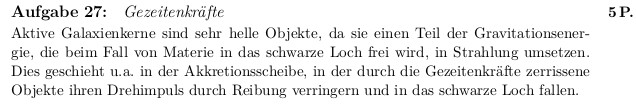
\includegraphics[width=\textwidth]{images/ex27_1.jpg}
\end{figure}
\begin{figure}[H]
    \centering
    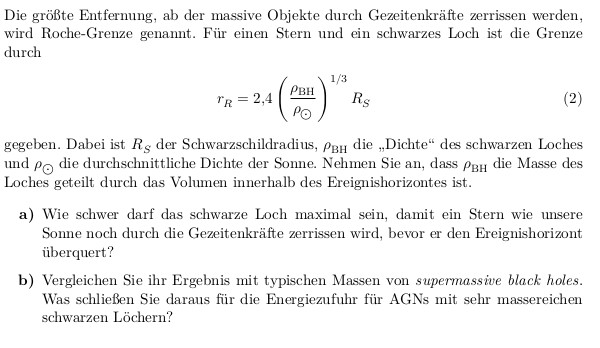
\includegraphics[width=\textwidth]{images/ex27_2.jpg}
\end{figure}



\subsection{a)}
\flushleft{Um\;}\justifying die Maximale Masse, für die die Gezeitenkräfte  massive Objekte vor Überschreitung des Ereignishorizonts
zerreißen, zu bestimmen, wird die Formel (2) am Radius des Ereignishorizonts untersucht.
\begin{align}
    R_S &= 2,4 \left( \frac{\rho _{BH}}{\rho _{\odot}} \right)^{\frac{1}{3}} R_S \\
    \rho _{BH} &= \frac{M_{BH}}{V_{BH}} = \frac{M_{BH}4}{3 \pi R_S^3}\\
    \intertext{
        Der Schwarzschildradius berechnet bei einem stationären schwarzen Loch durch
    }
    R_S &= \frac{2GM_{BH}}{c^2}\\
    \rho_{BH} &= \frac{ c^6}{6 \pi G^3 M_{BH}^2} \\
    \intertext{weiter mit der Hauptrechnung}
    1 &= (2,4)^3 \left( \frac{c^6}{6 \pi G^3 M_{BH}^2 \rho _{\odot}} \right)\\
    M_{BH} &= \sqrt{ \frac{549 c^6}{500 \pi G^3 \rho _{\odot} } }\\
    M_{BH} &= \text{\input{M_BH.tex}}
    \intertext{
        Damit ergibt sich eine Obergrenze für die Masse von
    }
    M_{BH} \leq  \text{\input{M_BH.tex}}, \label{eq:8}
\end{align}
damit die Gezeitenkräfte vor Übertretung des Ereignishorizonts die Masse zerreißen.

\subsection{b)}
\flushleft{Typische\;}\justifying Massen von supermassiven schwarzen Löchern liegen in Größenordnungen von
$10^5\-- 10^{10} M_{\odot} $. Bei schwarzen Löchern, die in die Grenze nach Gleichung
\eqref{eq:8} fallen, wird die Energie außerhalb des Ereignishorizonts frei und
landet nicht zwangsweise im schwarzen Loch. Bei schwarzen Löchern mit höheren Massen
findet die Zerreißung erst innerhalb des Ereignishorizonts statt und die gesamte Energie
bleibt im schwarzen Loch. Dadurch würde ein Stern wie unsere Sonne keinen Beitrag zur 
Akkretionsscheibe liefern.



\end{document}
